\documentclass[a5paper]{article}
\usepackage[a5paper, top=8mm, bottom=8mm, left=8mm, right=8mm]{geometry}

\usepackage{polyglossia}
\setdefaultlanguage[babelshorthands=true]{russian}

\usepackage{fontspec}
\setmainfont{FreeSerif}
\newfontfamily{\russianfonttt}[Scale=0.7]{DejaVuSansMono}

\usepackage[font=scriptsize]{caption}

\usepackage{amsmath}
\usepackage{amssymb,amsfonts,textcomp}
\usepackage{color}
\usepackage{array}
\usepackage{hhline}
\usepackage{cite}

\usepackage[hang,multiple]{footmisc}
\renewcommand{\footnotelayout}{\raggedright}

\PassOptionsToPackage{hyphens}{url}\usepackage[xetex,linktocpage=true,plainpages=false,pdfpagelabels=false]{hyperref}
\hypersetup{colorlinks=true, linkcolor=blue, citecolor=blue, filecolor=blue, urlcolor=blue, pdftitle=1, pdfauthor=, pdfsubject=, pdfkeywords=}

\usepackage{tabu}

\usepackage{graphicx}
\usepackage{indentfirst}
\usepackage{multirow}
\usepackage{subfig}
\usepackage{footnote}
\usepackage{minted}
\usepackage{xcolor}

\newcommand{\attribution}[1] {
    \vspace{-5mm}\begin{flushright}\begin{scriptsize}\textcolor{gray}{\textcopyright\, #1}\end{scriptsize}\end{flushright}
}

\sloppy
\pagestyle{plain}

\title{Практика 4: моделирование структуры}
\author{Юрий Литвинов\\\small{yurii.litvinov@gmail.com}}

\date{07.02.2022}

\begin{document}

\maketitle
\thispagestyle{empty}

\section{Диаграммы классов}

Самая известная и самая частоиспользуемая диаграмма UML --- это, пожалуй, диаграмма классов. Про неё, конечно, подробно рассказывали на лекции, но тут обсудим частые ошибки начинающих проектировщиков. В целом её синтаксис хорошо проиллюстрирован в книжке М. Фаулера <<UML. Основы>> (кстати, книга очень рекомендуется как быстрая справка по UML, информации в которой вполне достаточно, чтобы успешно пользоваться языком):

\begin{center}
    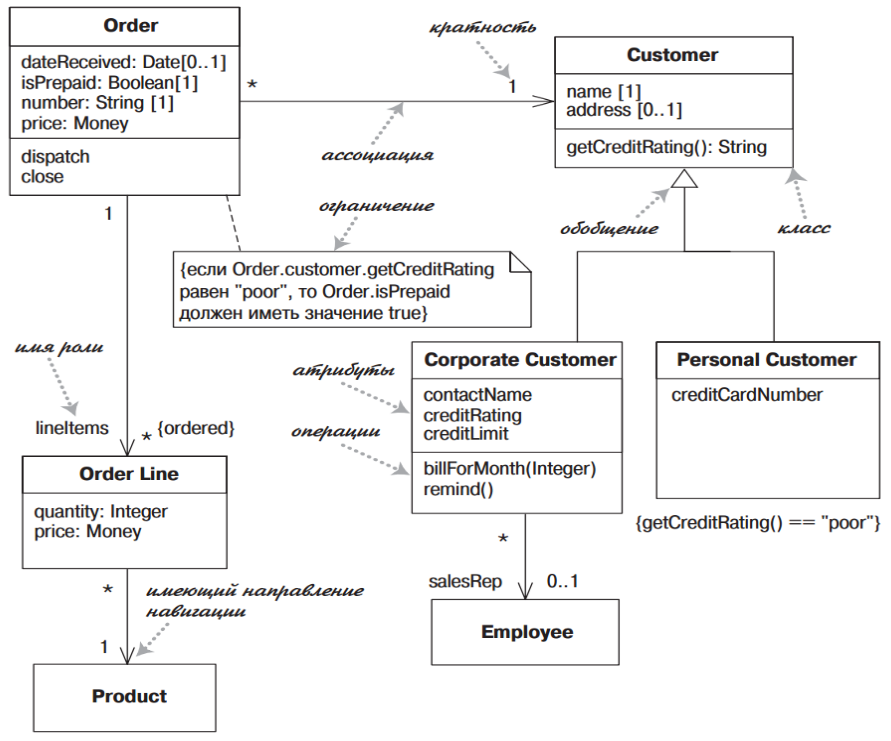
\includegraphics[width=0.8\textwidth]{umlClassDiagram.png}
    \attribution{М. Фаулер. <<UML. Основы>>}
\end{center}

На что обратить внимание:

\begin{itemize}
    \item наследование в UML называется <<обобщение>> (generalization) и стрелка указывает на предка, а не на потомка;
    \item кратность ассоциации тоже может вызвать путаницу, она пишется у того конца ассоциации, к которому относится кратность --- Customer может иметь много Order (звёздочка означает <<0 или больше>>), но у каждого Order ровно один Customer;
    \item все UML-диаграммы допускают не отображать некоторую информацию, если автор считает её не важной в данном контексте --- например, неверно, что класс Employee не имеет ни методов, ни полей, просто автор посчитал, что они не важны и решил не загромождать диаграмму.
\end{itemize}

\subsection{Атрибуты}

У диаграмм классов есть важная синтаксическая особенность --- атрибуты и ассоциации представляют собой с точки зрения синтаксиса языка одно и то же, просто отображаются по-разному. Например, диаграммы

\begin{center}
    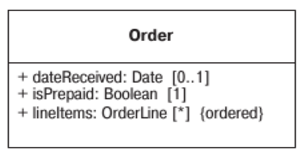
\includegraphics[width=0.3\textwidth]{attributes.png}
    \attribution{М. Фаулер. <<UML. Основы>>}
\end{center}

и

\begin{center}
    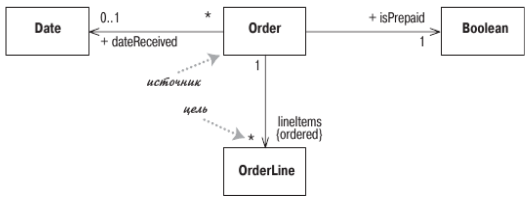
\includegraphics[width=0.7\textwidth]{associations.png}
    \attribution{М. Фаулер. <<UML. Основы>>}
\end{center}

означают в точности одно и то же. Атрибуты обычно используются, когда связи между классами не важны: когда типы атрибутов --- элементарные типы или перечисления (или даже структуры, короче, являются типами-значениями по смыслу; либо типы атрибутов --- это полноценные классы, но из третьесторонних библиотек). Ассоциации --- когда связи между классами важны для понимания архитектуры (чаще всего, когда типы атрибутов --- классы из реализуемой системы). На практике это означает, что:

\begin{itemize}
    \item не надо рисовать связи с enum-ами;
    \item если нарисовали связь, не пишите атрибут внутри класса;
    \item если поле два, рисуйте две ассоциации;
    \item не стесняйтесь именовать роли, указывать множественности и т.п.
\end{itemize}

\subsection{Агрегация и композиция}

Агрегация и композиция ---- дальнейшие уточнения ассоциации. На самом деле, если на диаграмме нарисована просто ассоциация, то при реализации мы вправе выбрать, агрегацию или композицию использовать. Разница между агрегацией и композицией --- во владении объектами, которые участвуют в ассоциации. Агрегация не предполагает владения:

\begin{center}
    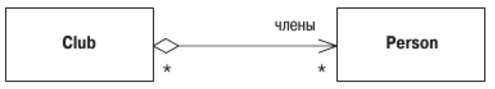
\includegraphics[width=0.5\textwidth]{aggregations.png}
\end{center}

Человек и клуб могут существовать независимо друг от друга, и когда закрывается клуб, его члены продолжают существовать (если это не тоталитарная секта). На диаграмме выше нарисовано, что в клубе может состоять несколько человек, и человек может состоять в нескольких клубах, при этом клуб знает о человеке, но не владеет им.

Композиция говорит, что один объект владеет другим объектом, то есть время их жизни связано и <<хозяин>> отвечает за удаление подчинённого ему объекта. Например, если мы пишем графический редактор, вполне может быть, что мы сделаем так:

\begin{center}
    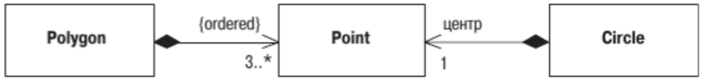
\includegraphics[width=0.7\textwidth]{compositions.png}
\end{center}

Здесь многоугольник состоит из точек, и когда мы удаляем многоугольник, удаляются и все точки, которые его определяют. Круг тоже имеет одну точку --- центр круга, и тоже, удаляем круг --- удаляется и его центр. Так что и круг и многоугольник владеют своими точками, но у каждой точки во время исполнения может быть только один хозяин.

Агрегация и композиция важны, если в итоге мы будем писать на C++ --- там они помогают следить за тем, кто в итоге должен освободить память из-под объекта. Для языков со сборкой мусора это не так важно (хотя и полезно знать, кто кем владеет), поэтому агрегация с композицией используются в диаграммах классов довольно редко --- обычно архитекторы ограничиваются ассоциациями, не специфицируя, агрегация эта конкретная ассоциация или композиция.

С точки зрения нотации надо запомнить, что агрегация --- более слабое отношение, чем композиция, поэтому и ромбик в случае агрегации не закрашен. И ромбики рисуются около контейнера (то есть клуб содержит людей, а не наоборот) --- можно понимать ромбик как оперение стрелы, указывающей от контейнера к содержащемуся в нём объекту. Ещё один небольшой пример:

\subsection{Остальное}

Интерфейсы: 

\begin{center}
    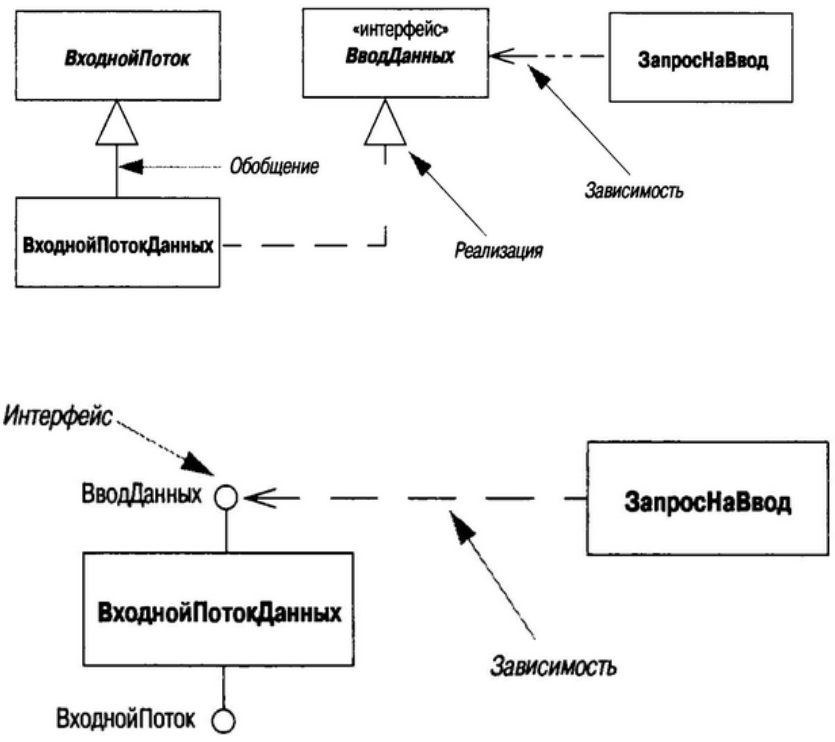
\includegraphics[width=0.6\textwidth]{interfaces.png}
    \attribution{М. Фаулер. <<UML. Основы>>}
\end{center}

Тут стоит помнить, что, так же, как в Java, реализация интерфейса и наследование от класса в UML суть разные вещи, реализация интерфейса рисуется пунктирной линией. Либо используется <<леденцовая>> нотация, когда реализуемый классом интерфейс рисуется как кружок с названием интерфейса, соединённый с классом линией. Такая нотация предпочтительней, если нам не очень важны методы интерфейса либо если интерфейсов много. Нотация со словом \verb|<<интерфейс>>| (или \verb|<<nterface>>| по-английски) используется, когда надо показать и методы интерфейса тоже (и тогда они пишутся как методы класса). Леденцовая нотация обычно используется на диаграмме компонентов, <<полная>> --- на диаграмме классов.

Зависимости:

\begin{center}
    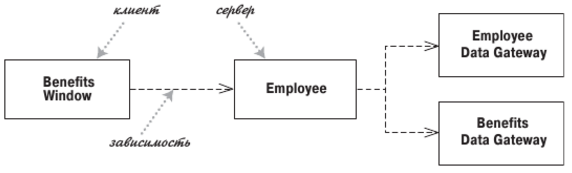
\includegraphics[width=0.7\textwidth]{dependencies.png}
    \attribution{М. Фаулер. <<UML. Основы>>}
\end{center}

Вообще зависимость--- наиболее общий вид связи между классами, она означает просто, что один класс (или интерфейс) что-то знает про другой (например, он ему нужен, чтобы скомпилироваться). Зависимости могут быть уточнены стереотипами, некоторые из которых прописаны в стандарте:

\begin{itemize}
    \item call --- один класс вызывает метод другого;
    \item create или instantiate--- один класс создаёт в каком-то из своих методов объект другого;
    \item derive --- однин класс представляет значение, которое может быть вычислено по другому;
    \item realize --- один класс реализует другой (например, абстрактный класс);
    \item responsibility --- контракт, который класс обязуется исполнять;
    \item refine --- зависимость, которая может быть установлена даже между элементами с разных диаграмм, один элемент является уточнением другого --- например, класс из модели предметной области уточняется набороом классов из реализации;
    \item trace --- зависимость, которая может быть установлена даже между элементами с разных диаграмм, означает, что один элемент как-то влияет на другой --- например, случай использования может быть связан отношением trace с классами, которые его реализуют. Нужны такие зависимости прежде всего для автоматического отслеживания изменений.
\end{itemize}

Со стереотипами зависимости рисуются так:

\begin{center}
    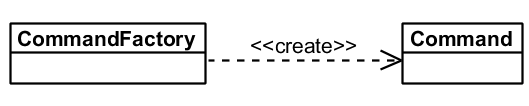
\includegraphics[width=0.4\textwidth]{createDependency.png}
\end{center}

Обратите внимание на <<ёлочки>>, это часть синтаксиса языка.

Шаблоны и перечисления:

\begin{center}
    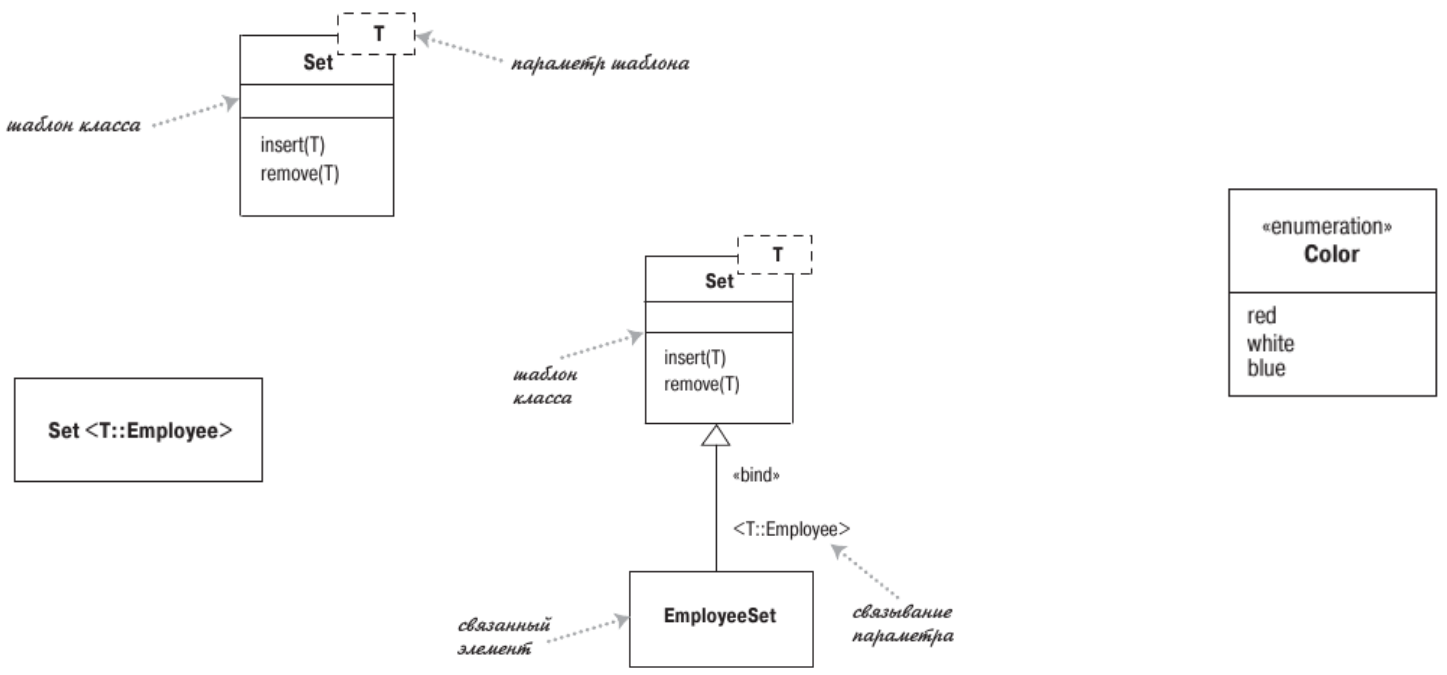
\includegraphics[width=\textwidth]{genericsAndEnums.png}
    \attribution{М. Фаулер. <<UML. Основы>>}
\end{center}

В отличие от первых версий Java, в UML синтаксис для шаблонных классов (или генериков) был всегда: параметры-типы перечисляются через запятую в пунктирном прямоугольнике в правом верхнем углу класса. Инстанцирование шаблона (то есть подстановка фактических параметров-типов вместо формальных) рисуется либо как просто класс, у которого указано, что куда подставляется, либо как наследование со стереотипом \verb|<<bind>>|, как на рисунке.

Второй способ используется, когда экземпляр шаблона доопределяет ещё какие-нибудь методы и поля (например, классы QList<T> и QStringList в библиотеке Qt, второй является специализацией первого для типа QString, но добавляет ещё специфичные методы, например, join()).

На рисунке также видно, как задаются перечисления. Используется стереотип \verb|<<enumeration>>| и просто перечисляются элементы.

\section{Диаграммы компонентов}

Диаграммы компонентов --- пожалуй, самые полезные для архитектора диаграммы UML. На них изображаются компоненты, из которых состоит система или подсистема, и взаимосвязи между ними. Точного определения термина <<компонент>> не существует, но все интуитивно представляют, что это такое --- нечто структурно связанное и больше, чем класс. Компонентами могут быть пакеты, пространства имён, сборки, .dll/.so-файлы, отдельные веб-сервисы в распределённом приложении и т.д. В общем, это именно то, из чего состоит высокоуровневая архитектура приложения.

Полезны диаграммы компонентов как вид <<с высоты птичьего полёта>> на создаваемую систему. Например, вот диаграмма, описывающая высокоуровневую архитектуру проекта QReal (\url{https://github.com/qreal/qreal}, инструмент для создания визуальных предметно-ориентированных языков и работы с ними):

\begin{center}
    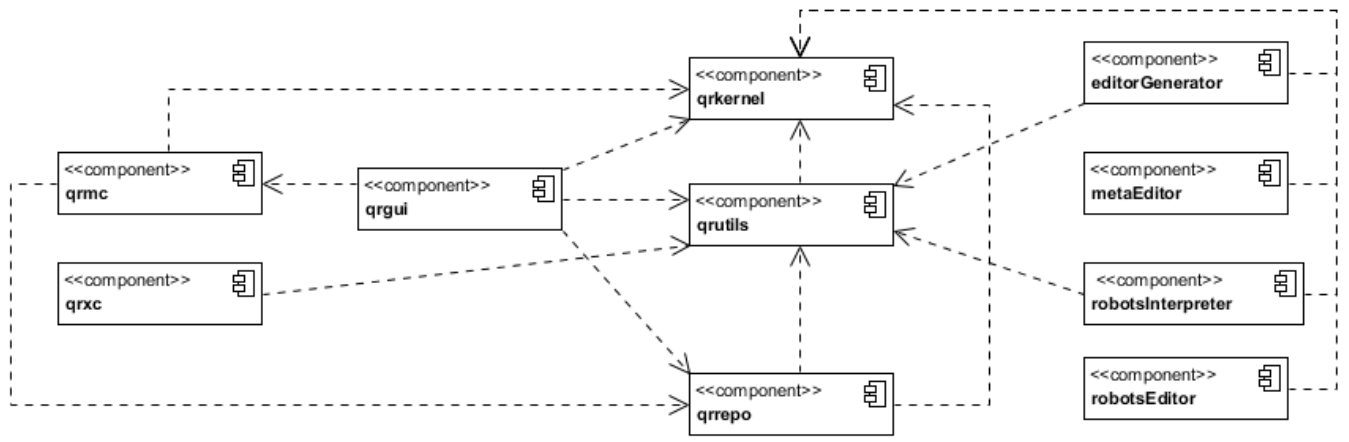
\includegraphics[width=0.95\textwidth]{componentDiagrams.png}
\end{center}

Связи между компонентами тут означают зависимости по сборке, каждый компонент --- это отдельный проект, который собирается в отдельный .dll/.so-файл. По такой диаграмме можно очень быстро рассказать общую архитектуру проекта: qrkernel ни от кого не зависит, там находятся классы, общие для всей системы; qrutils содержит полезную функциональность, используемую в других модулях; qrrepo --- репозиторий, где хранятся данные, с которыми QReal работает; qrgui --- пользовательский интерфейс; qrmc и qrxc --- это компиляторы визуальных языков, с которыми работает Real; editorGenerator, metaEditor, robotsInterpreter, robotsEditor --- это плагины инструментальной поддержки работы с визуальными языками. Конечно, это не полноценное архитектурное описание, но даже этого достаточно, чтобы было понятно, куда смотреть в исходниках.

Вот описание синтаксиса диаграмм компонентов, на сей раз с сайта \url{http://www.uml-diagrams.org} (очень рекомендую, как быструю справку по синтаксису и как набор примеров с пояснениями):

\begin{center}
    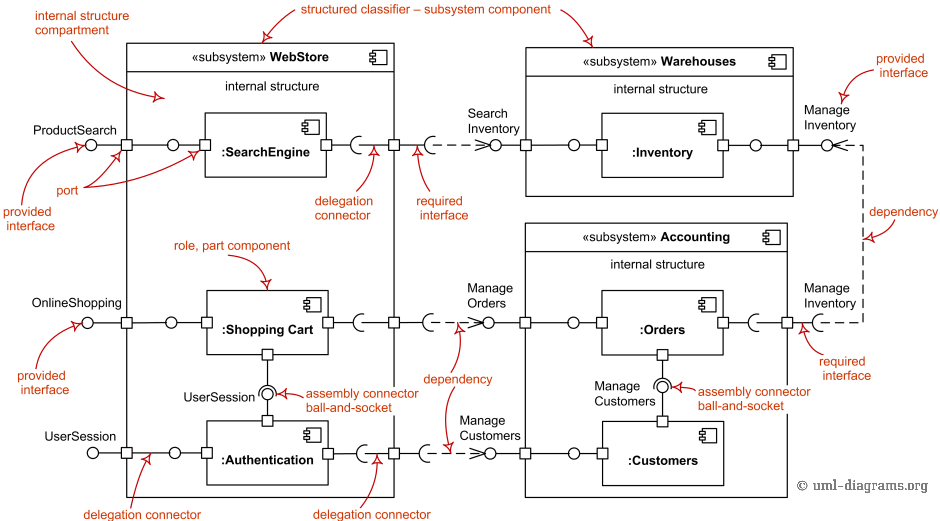
\includegraphics[width=0.95\textwidth]{componentDiagramsOverview.png}
    \attribution{\url{http://www.uml-diagrams.org}}
\end{center}

Видно, что компоненты могут быть вложенными друг в друга, что они могут иметь интерфейсы (так же, как и классы, но на диаграммах компонентов чаще всего используется только <<леденцовая>> нотация). У компонентов есть порты, которые могут предоставлять или потреблять интерфейсы, но порты часто не рисуются, а подразумеваются, поскольку обычно порт имеет только один интерфейс. Порты бывают полезны для изображения делегирования --- что компонент просто перенаправляет запросы вложенному компоненту. Слова \verb|<<subsystem>>| и <<internal structure>> опциональны (и обычно не пишутся).

\section{Диаграмма развёртывания}

Вот пример и напоминание синтаксиса диаграммы развёртывания, из книжки Фаулера:

\begin{center}
    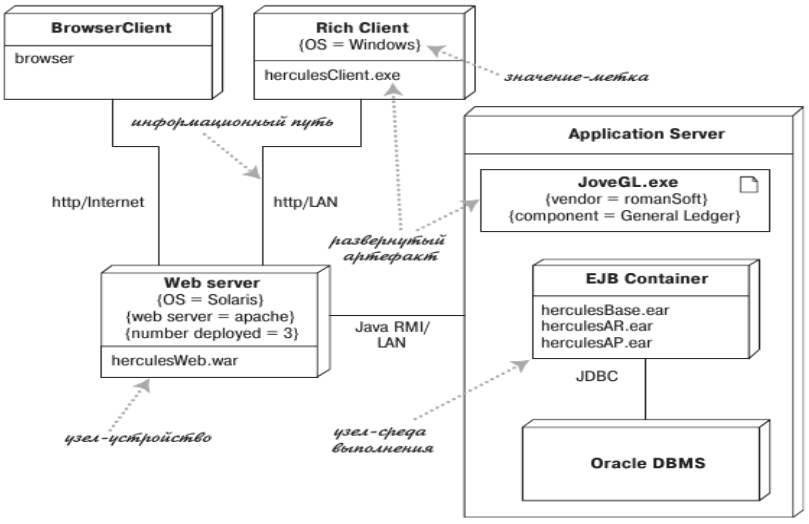
\includegraphics[width=0.7\textwidth]{deploymentDiagram.png}
    \attribution{М. Фаулер, UML. Основы}
\end{center}

На что стоит обратить внимание:

\begin{itemize}
    \item связи тут показывают не логическую связь между артефактами, а каналы между узлами (как правило, физические, хотя и может быть что-то вроде VPN); грубо говоря, это не <<кто кого вызывает>>, а <<провода>>, которыми связаны узлы;
    \item просто узлы рисовать бесполезно, надо показать, что на них развёрнуто --- чаще всего рисуют \emph{артефакты}, то есть единицы развёртывания типа .exe, .so, .jar-файлов, но можно рисовать и компоненты (и это часто более полезно, позволяет понять, как логическая функциональность распределена по физическим устройствам);
    \item связи между компонентами не рисуют вовсе --- на то есть диаграмма компонентов;
    \item стоит указывать характеристики узлов, если они важны/известны, в частности, множественность.
\end{itemize}

\section{Задание на остаток пары}

Вспомнить запрос \url{https://bit.ly/defects-rfp}, подумать над тем, как бы вы стали делать такую систему, и построить по нему:

\begin{enumerate}
    \item диаграмму классов, моделирующую данные, хранимые системой;
    \item диаграмму компонентов требуемой системы, как вы её видите;
    \item диаграмму развёртывания, как вы её видите;
    \begin{itemize}
        \item с указанием компонентов, разворачиваемых на узле;
    \end{itemize}
\end{enumerate}

Постарайтесь уложиться в оставшееся время, так что не стоит увлекаться подробностями.

\end{document}